\chapter{Introduction}
\label{Chapter1}
\lhead{Chapter 1. \emph{Introduction}}

A production Kubernetes node shares a single Linux kernel among tens to
hundreds of containers. That kernel is a shared fate~\cite{gregg2019bpf}: one
race in namespace teardown, one off-by-one in \texttt{copy\_from\_user}, one
exploitable path in \texttt{io\_uring}---any of these hands every co-tenant on
the node to the attacker at once. Container isolation is a policy, not a
hardware boundary. It holds until it does not.

This thesis is about the attacks that never need to break that boundary. They
walk between containers through syscalls the kernel is already allowed to
serve. Each hop reads as benign under any local per-container policy, yet the
composition is a credential exfiltration, a lateral pivot, a container
escape. The work reported here builds a three-tier runtime defence that
treats such compositions as first-class: not deviations from a single
container's profile, but \emph{edges} in a graph that the kernel can
instrument directly.

%─────────────────────────────────────────────────────────────────────────────
\section{The shared-kernel attack surface}
\label{sec:attack-surface}
%─────────────────────────────────────────────────────────────────────────────

Modern microservice deployments layer an externally reachable tier (a web
front-end, an API gateway) over an internal tier (databases, caches, message
queues) that the outer tier reaches over a flat overlay network. Both layers
share the same kernel, the same cgroup hierarchy, and the same BPF map space.

Consider a concrete chain on the evaluation testbed: \texttt{ct\_attacker}
exploits a server-side request forgery in \texttt{ct-nginx}, which proxies a
crafted request to \texttt{ct-api-gw} on port 8080. The gateway, processing
what it reads as a legitimate upstream call, queries \texttt{ct-postgres} on
port~5432. Each individual syscall along the way---\texttt{connect(2)},
\texttt{sendmsg(2)}, \texttt{recvmsg(2)}---is permitted by any reasonable
per-container policy. The anomaly lives entirely in the \emph{edge} between
containers, not in any single container's syscall trace.

Existing open-source defences miss this class of attack by design.
Falco~\cite{falco2024} matches per-container syscall sequences against a rule
library; it fires on payloads. Tetragon~\cite{tetragon2024} attaches kprobes
and enforces per-pod network policies. Tracee~\cite{tracee2024} builds
per-process behaviour profiles. None of the three model the relationship
\emph{between} containers.

%─────────────────────────────────────────────────────────────────────────────
\section{Why per-container detectors are blind to composite attacks}
\label{sec:bosc-blindness}
%─────────────────────────────────────────────────────────────────────────────

The dominant IDS paradigm for containers is a variant of
Bag-of-System-Calls~(BoSC)~\cite{bertinatto2024,kotenko2024}: build a
frequency or sequence profile of the syscalls a container issues under normal
operation, then flag deviations at runtime. These detectors are lightweight
and interpretable. Their weakness is semantic. They observe \emph{what} a
container does, not \emph{why} or \emph{in response to whom}.

We showed this empirically during mid-review. The same
\texttt{openat("/etc/passwd")} is benign when \texttt{apt-get} resolves a
user-ID and malicious when a compromised worker reads credentials. The same
\texttt{clone(2)} burst is benign when \texttt{gpgv} verifies package
signatures and malicious during a fork bomb. The same \texttt{setuid(0)} is
required by \texttt{runc} during container init and forbidden during request
handling~\cite{ghimire2025patrol}. Every benign case forces a whitelist entry into
any rule-based detector. Every whitelist entry becomes an evasion vector.

The deeper failure mode is multi-hop composition. Suppose an attacker chain
runs: shell spawn in \texttt{ct-webapp-a}, lateral connect to
\texttt{ct-api-gw} on an uncalibrated port, further connect to
\texttt{ct-postgres}~\cite{he2023cross}. Each container produces a locally
plausible trace. The attack is encoded in the \emph{joint} behaviour of the
trio---in the fact that the shell-spawn and the lateral connect occurred
inside the same five-second window in the same cgroup, and that the
downstream container then opened a connection it had never opened during
calibration. Standard BoSC tooling cannot see that joint behaviour; it lacks
the mathematical object---a global model of how containers are \emph{supposed
to} couple---that would encode it.

\begin{figure}[t]
  \centering
  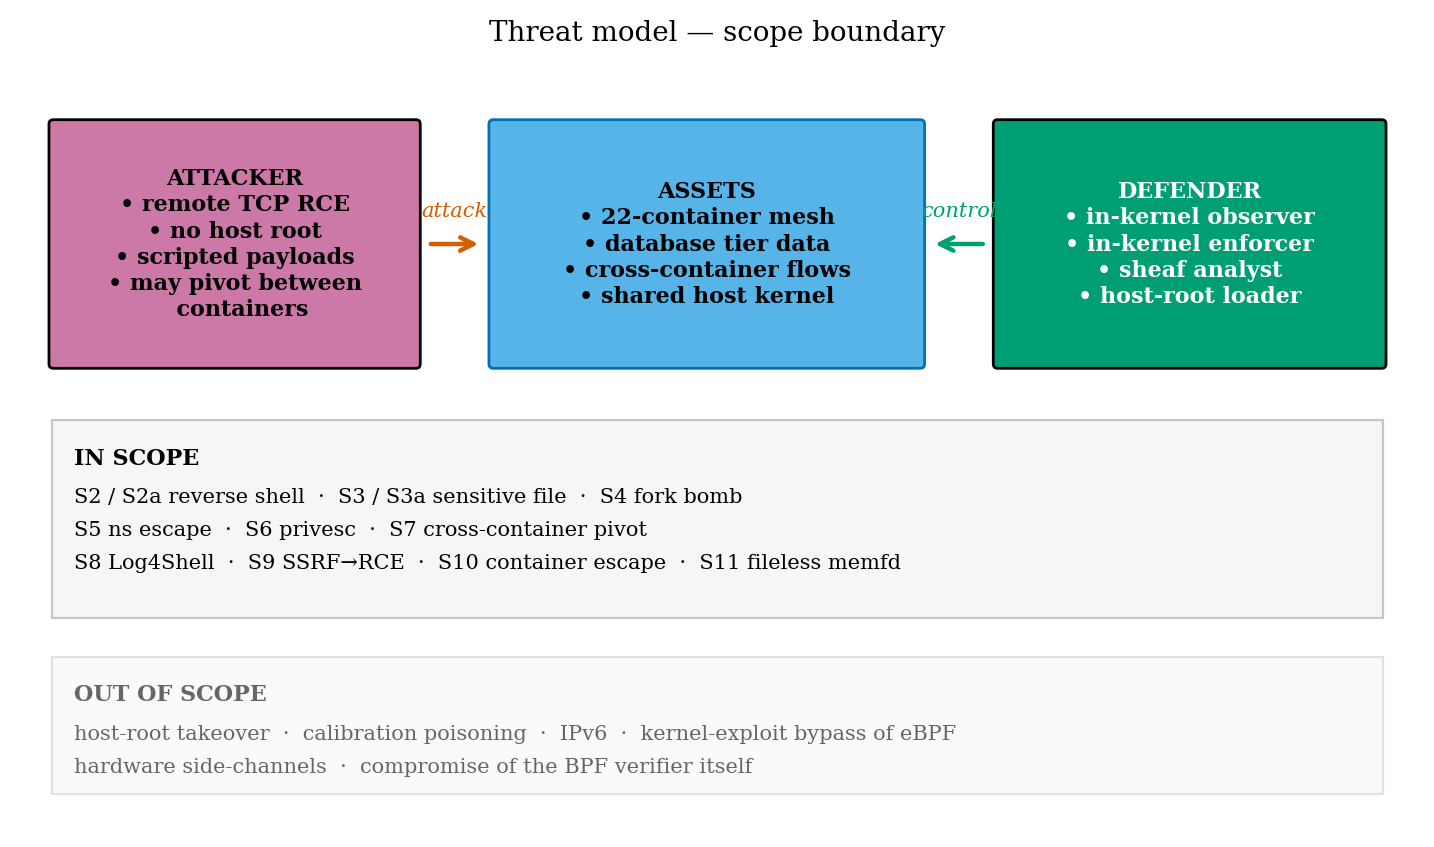
\includegraphics[width=0.92\linewidth]{figures/fig_threat_model.png}
  \caption[Thesis scope boundary]{Scope of the defence. Every attack in the
  in-scope band is either a physical kernel invariant (caught by Tier~1) or a
  cross-container edge anomaly (caught by Tier~3). The out-of-scope band lists
  assumptions that are standard for this class of system.}
  \label{fig:intro-scope}
\end{figure}

%─────────────────────────────────────────────────────────────────────────────
\section{Problem statement}
\label{sec:problem}
%─────────────────────────────────────────────────────────────────────────────

\textbf{Problem.} Design, implement, and evaluate a container security
system that
\begin{enumerate}
  \item enforces physical syscall invariants at sub-microsecond latency with
        no user-space decision in the kill path,
  \item attributes every accepted network byte to the client IP that caused
        it, so enforcement is \emph{surgical}---one attacker IP is severed
        rather than the entire container process being killed,
  \item detects novel cross-container attack chains that no per-container
        IDS can see, using a principled mathematical model of inter-container
        coupling, and
  \item sustains a realistic concurrent workload with measurable, bounded
        overhead, producing detection rates with tight confidence intervals
        against Falco and Tetragon baselines on the same host.
\end{enumerate}

%─────────────────────────────────────────────────────────────────────────────
\section{Contributions}
\label{sec:contributions}
%─────────────────────────────────────────────────────────────────────────────

This thesis makes four contributions.

\paragraph{A three-tier architecture with a strict dependency rule.}
Tier~1 (kernel, 6 eBPF handlers) enforces kernel invariants inline on
\texttt{sys\_enter}. Tier~2 (kprobe on \texttt{inet\_csk\_accept} plus a TC
classifier) attributes every accepted byte to a client IP and severs the
attacker session at the veth by dropping their packets on an expiring BPF
map. Tier~3 (Python daemon) computes a 74-dimensional signal per container
per five-second window and passes it through a cellular sheaf Laplacian. The
dependency rule is asymmetric: Tier~1 never blocks on Tier~3.

\paragraph{TC-drop session severance.}
Earlier prototypes called \texttt{bpf\_send\_signal(9)} against the container
process, which terminated every live connection the container was serving.
We replace this with a \texttt{drop\_ip\_list} BPF map (key: IPv4 source,
value: \texttt{CLOCK\_MONOTONIC} expiry) read by the TC ingress and egress
classifiers on each veth. Only packets to or from the burned IP are dropped;
other clients are untouched. A five-minute TTL self-heals false positives
without operator intervention.

\paragraph{A rank-15 CCA calibration that fits real calibration windows.}
An earlier iteration of the pipeline fitted CCA at $k=50$ and produced
rank-deficient restriction maps whenever a calibration window contained
fewer than sixty aligned samples per edge. We show that $k=15$ keeps every
edge well-conditioned at realistic calibration durations on our 22-container
testbed and eliminates the false-positive storm that a rank-deficient
covariance inversion causes at runtime.

\paragraph{A seed-reproducible evaluation harness.}
A fixed random permutation of 150 in-distribution attack injections (drawn
from eleven classes) plus five held-out \texttt{memfd\_create} out-of-
distribution injections is replayed identically against CausalTrace, Falco
(stock and tuned), and Tetragon (stock and tuned) under the same concurrent
background load. The harness produces per-scenario Wilson 95\,\% confidence
intervals~\cite{wilson1927}, detection-latency cumulative distributions, and
per-syscall overhead. Chapter~\ref{Chapter6} reports the results.
